\vspace{-0.2cm}
\section{Learning Policies for New Tasks from Offline RL Pre-training}
\label{sec:ptr_method}
\vspace{-0.2cm}

To effectively solve new tasks from diverse offline datasets, a robotic learning framework must: \textbf{(1)} extract useful skills out of the diverse robotic dataset, and \textbf{(2)} rapidly specialize the learned skills towards an unseen target task, given only a minimal amount of experience from this target task in the form of demonstrations, or collected autonomously by interaction. In this section, we present our framework, \ptrmethodname, that provides these benefits by training a single, highly expressive deep network via offline RL, and then specializes it on the target task with a small amount of data. We will first present the key components of our robotic framework in Section~\ref{sec:ptr_algorithm} and then discuss our novel technical contributions, the practical design choices that are crucial, in Section~\ref{sec:design_choices}.    

\begin{figure}
  \centering
  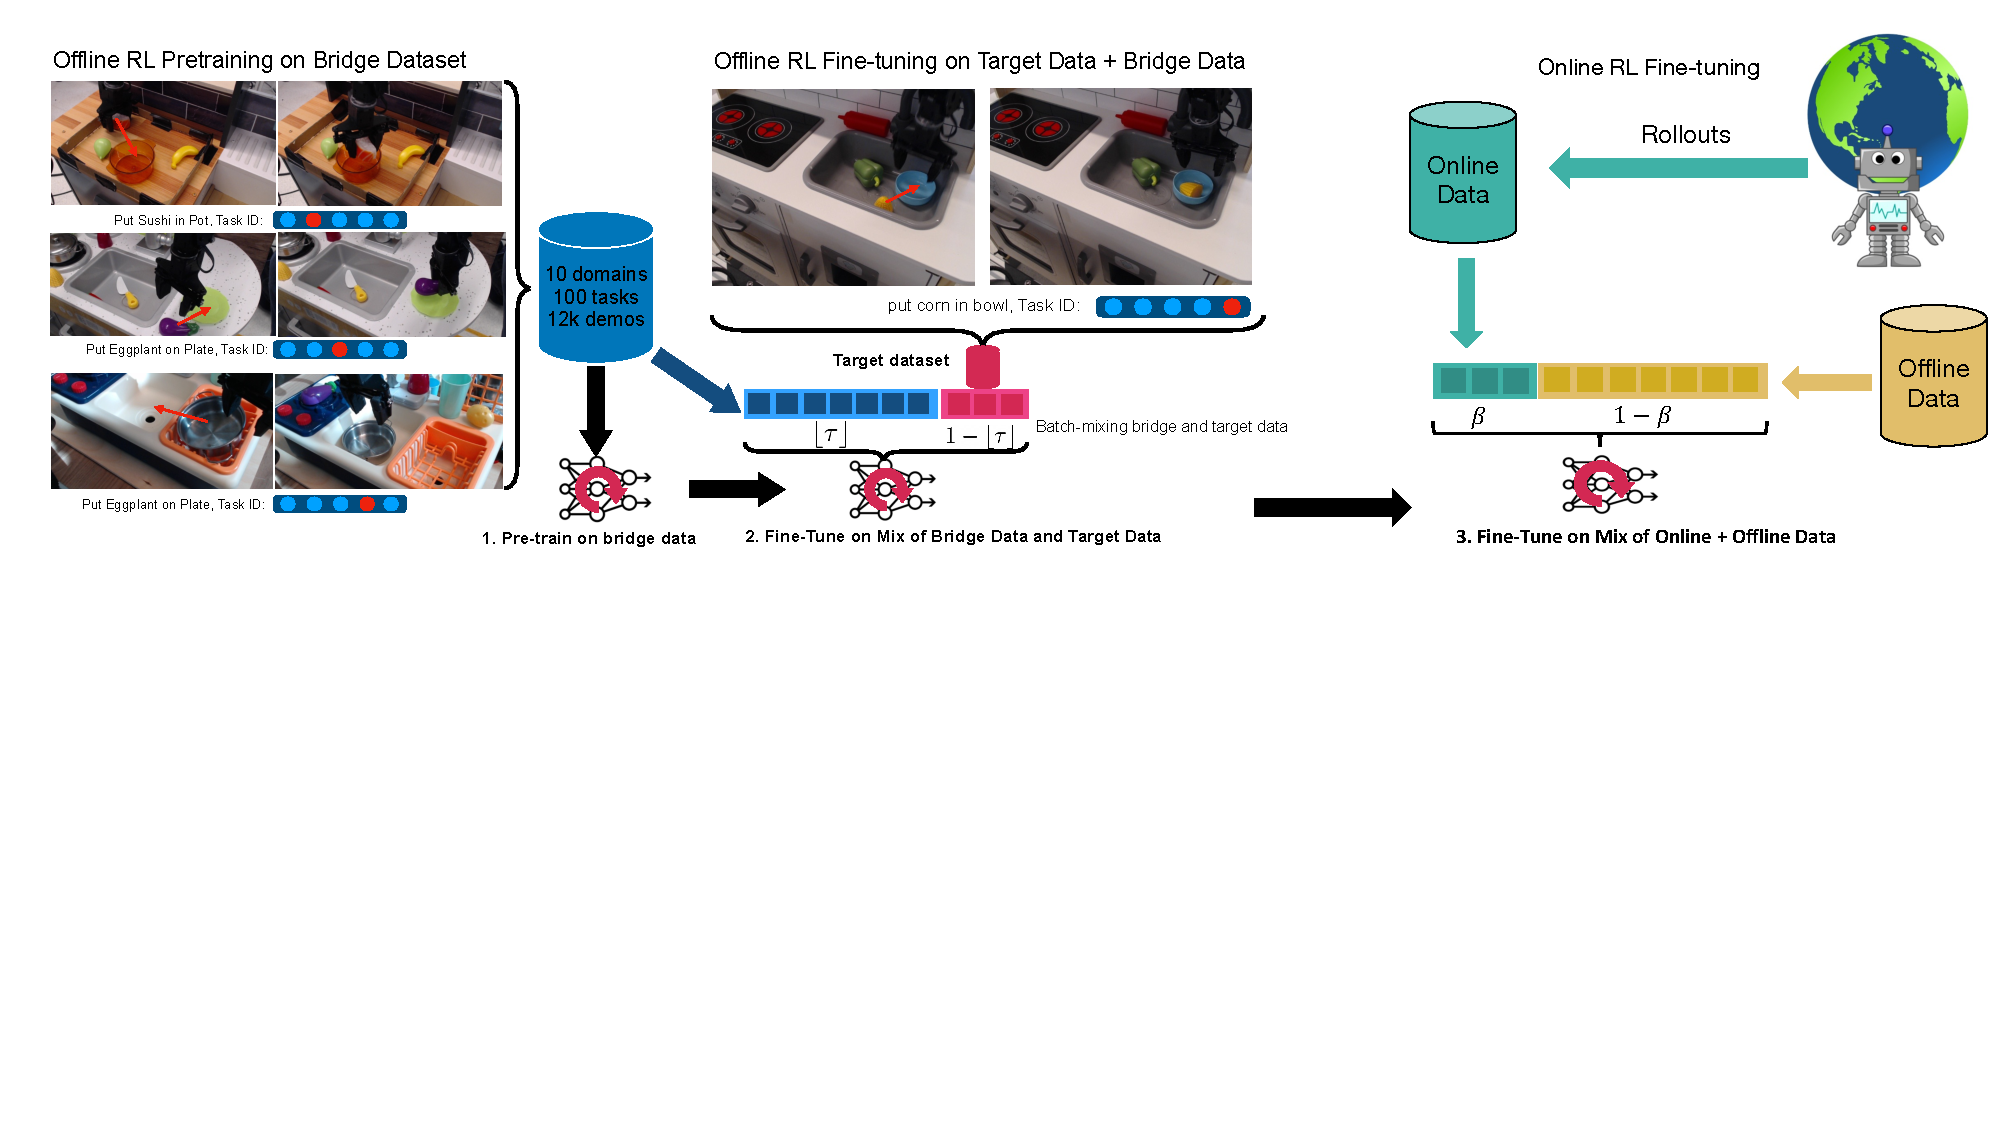
\includegraphics[width=1.0\linewidth]{chapters/ptr/system_overview.pdf}
  \vspace{-0.3cm}
  \caption{ \label{fig:system_overview} \footnotesize \textbf{Overview of \ptrmethodname:} We first perform general offline pre-training on diverse multi-task robot data and subsequently fine-tune on one or several target tasks while mixing batches between the prior data and the target dataset using a batch mixing ratio of $\tau$. Additionally, a separate online fine-tuning phase can be done, where offline pre-training is done on a static dataset and an online replay buffer is collected using rollouts in the environment. The offline and online buffers are mixed per batch with a ratio of $\beta$.}
  \vspace{-0.3cm}
\end{figure}

\vspace{-0.2cm}
\subsection{The Components of \ptrmethodname}
\label{sec:ptr_algorithm}
\vspace{-0.2cm}

To satisfy both requirements \textbf{(1)} and \textbf{(2)} from above, our framework uses a multi-task offline RL approach with parameter sharing, where the policy and Q-function are conditioned on a task identifier. This allows us to share a single set of weights for all possible tasks in the diverse offline dataset, providing a general-purpose pre-training procedure that can use diverse data. 
Once a policy is obtained via this multi-task pre-training process, we adapt this policy for solving a new target task by utilizing a very small amount of target task data or autonomously collected data. We describe the two phases, pre-training and fine-tuning, below:

\niparagraph{\textbf{Phase 1:} Multi-task offline RL pre-training.} In the first phase, \ptrmethodname learns a single Q-function and policy for all tasks $i \in \mathcal{T}_\text{train}$ conditioned on the task identifier $i$, i.e., $Q_\phi(\bs, \mathbf{a}; i)$ and $\pi_\theta(\mathbf{a}|\bs, i)$, via multi-task offline RL. We use a one-hot task identifier that imposes minimal assumptions on the task structure. For multi-task offline RL, we use the conservative Q-learning (CQL)~\citep{kumar2020conservative} algorithm. Recall that this amounts to training the multi-task Q-function against a temporal difference error objective along with a regularizer that explicitly minimizes the expected Q-value under the learned policy $\pi_\theta(\mathbf{a}|\bs; i)$,
to prevent overestimation of Q-values for unseen actions, which can lead to poor offline RL performance~\citep{kumar2019stabilizing}. 
% Formally, the training objective for our multi-task Q-function, as prescribed by CQL, is given by:
% \begin{align*}
% \label{eqn:cql_training}
% \!\!\!\!\!\!\!\! \min_{\phi}~~ & \alpha\left(\mathop{\mathbb{E}}_{\substack{i \sim \mathcal{T}_\text{train},\\ \bs \sim \mathcal{D}_i, \mathbf{a} \sim \pi}} \!\!\!\!\left[Q_\phi(\bs,\mathbf{a}; i)\right] - \!\!\!\mathop{\mathbb{E}}_{\substack{i \sim \mathcal{T}_\text{train},\\ \bs, \mathbf{a} \sim \mathcal{D}}}\!\!\!\left[Q_\phi(\bs,\mathbf{a}; i)\right]\right) \\ 
% & + \frac{1}{2} \mathop{\mathbb{E}}_{\substack{i \sim \mathcal{T}_\text{train},\\ \bs, \mathbf{a}, \bs' \sim \mathcal{D}\\\mathbf{a}' \sim \pi}}\left[\left(Q_\phi(\bs, \mathbf{a}; i) - r - \gamma Q_{\mathbf{a}r{\phi}}(\bs', \mathbf{a}')\right)^2 \right].
% \end{align*}  
% ${Q}_{\mathbf{a}r{\phi}}$ denotes the target Q-network, which is a delayed copy of the current Q-network. We train $\phi$ by running gradient descent on the above objective, and then optimize the learned policy to maximize the learned Q-values, along with an additional entropy regularizer as shown below:
% \begin{align*}
%     \max_{\theta}~~~~ \mathbb{E}_{{i \sim \mathcal{T}_\text{train}, \bs \sim \mathcal{D}_i}}\left[ \mathbb{E}_{\mathbf{a} \sim \pi_\theta(\cdot|\bs; i)}[Q_\phi(\bs, \mathbf{a}; i)]  \right] + \beta \mathcal{H}(\pi_\theta).
% \end{align*}
At the end of multi-task offline training phase, we obtain a policy $\pi^\text{off}_\theta$ and Q-function $Q^\text{off}_\phi$, that are ready to be fine-tuned to a new downstream task.

\niparagraph{\textbf{Phase 2: Offline or online fine-tuning of $\pi^\text{off}_\theta$ and $Q^\text{off}_\phi$ to a target task $\mathcal{T}_\text{target}$.}} In the second phase, PTR attempts to learn a policy to solve one or more downstream tasks by adapting $\pi^\text{off}_\theta$, using a limited set of user-provided demonstrations that we denote $\mathcal{D}^*$, or using a combination of target demonstration data and autonomously collected online data. Our method for the offline fine-tuning setting is simple yet effective: we incorporate the new target task data into the replay buffer of the very same offline multi-task CQL algorithm from the previous phase and resume training from Phase 1. However, na\"ively incorporating the target task data into the replay buffer might still not be effective since this scheme would hardly ever train on the target task data during adaptation due to the large imbalance between the sizes of the few target demonstrations and the large pre-training dataset. To address this imbalance, each minibatch passed to multi-task CQL during offline fine-tuning consists of a $\tau$ fraction of transitions from bridge demonstration data and $1 - \tau$ fraction of transitions from the target dataset. By setting $\tau$ to be small, we are able to prioritize multi-task CQL to look at target task data frequently, enabling it to make progress on the downstream task without overfitting.

For the autonomous fine-tuning, we utilize a similar technique and have each mini-batch consist of $\beta$ fraction of transitions from the bridge data and the target demonstration data, and $1 - \beta$ fraction of transitions from the newly collected online data. We alternate between collecting one trajectory and making 10 gradient steps for every single transition collected in the environment. Utilizing a high update to the data ratio allowed us to efficiently train the agent on newly collected online samples from rollouts.

\niparagraph{\textbf{Handling task identifiers for new tasks.}} The description of our system so far has assumed that the downstream test tasks are identified via a task identifier. In practice, we utilize a one-hot vector to indicate the index of a task. While such a scheme is simple to implement, it is not quite obvious how we should incorporate new tasks with one-hot task identifiers. In our experiments, we use two approaches for solving this problem: first, we can utilize a larger one-hot encoding that incorporates tasks in both $\mathcal{T}_\text{train}$ and $\mathcal{T}_\text{target}$, but not use the indices for $\mathcal{T}_\text{target}$ during pre-training. The Q-function and the policy are trained on these \emph{placeholder} task identifiers only during fine-tuning in Phase 2. 
Another approach for handling new tasks is to not use unique task identifiers for every new task, but rather ``\emph{re-target}'' or re-purpose existing task identifiers for new target tasks in the fine-tuning phase. \ptrmethodname provides this option: we can simply assign an already existing task identifier to the target demonstration data before fine-tuning the learned Q-function and the policy. For example, in our experiments in Section~\ref{sec:result} we re-target the put sushi in pot task which uses orange transparent pots to instead put the sushi into a metal pot, which was never seen during training.

An overview of our approach is shown in \autoref{fig:system_overview}. We use a value of $\alpha=10.0$ and $\tau=0.8$ for mixing the pre-training dataset and the target dataset in most of our experiments in the real-world, without requiring any domain-specific tuning. For online fine-tuning, we utilized $\alpha=0.5$ to evenly mix between the online and offline datasets. 

\vspace{-0.2cm}
\subsection{Important Design Choices and Practical Considerations}
\label{sec:design_choices}
\vspace{-0.2cm}
Even though the components discussed in Section~\ref{sec:ptr_algorithm} are sufficient to give rise to an offline pre-training and fine-tuning approach, as we show in Section~\ref{fig:experiments}, this approach does not lead very good results on its own. Instead, we must make some crucial design decisions, including designing  neural network architectures that can learn from diverse data with offline RL,
cross-validation metrics to identify policies we expect to be effective after fine-tuning, and the design of the reward functions that can be used to label the pre-training dataset. {We show that making the right choices for these components leads to significant improvement (more than \textbf{3.5x} in final real-world performance; see Appendix~\ref{app:design}). Thus, describing, analyzing, and evaluating these choices is a crucial part of this work that we hope will facilitate applications of offline RL pre-training.}


\begin{figure}
\vspace{-0.5cm}
    \centering
    \setcounter{figure}{1}
  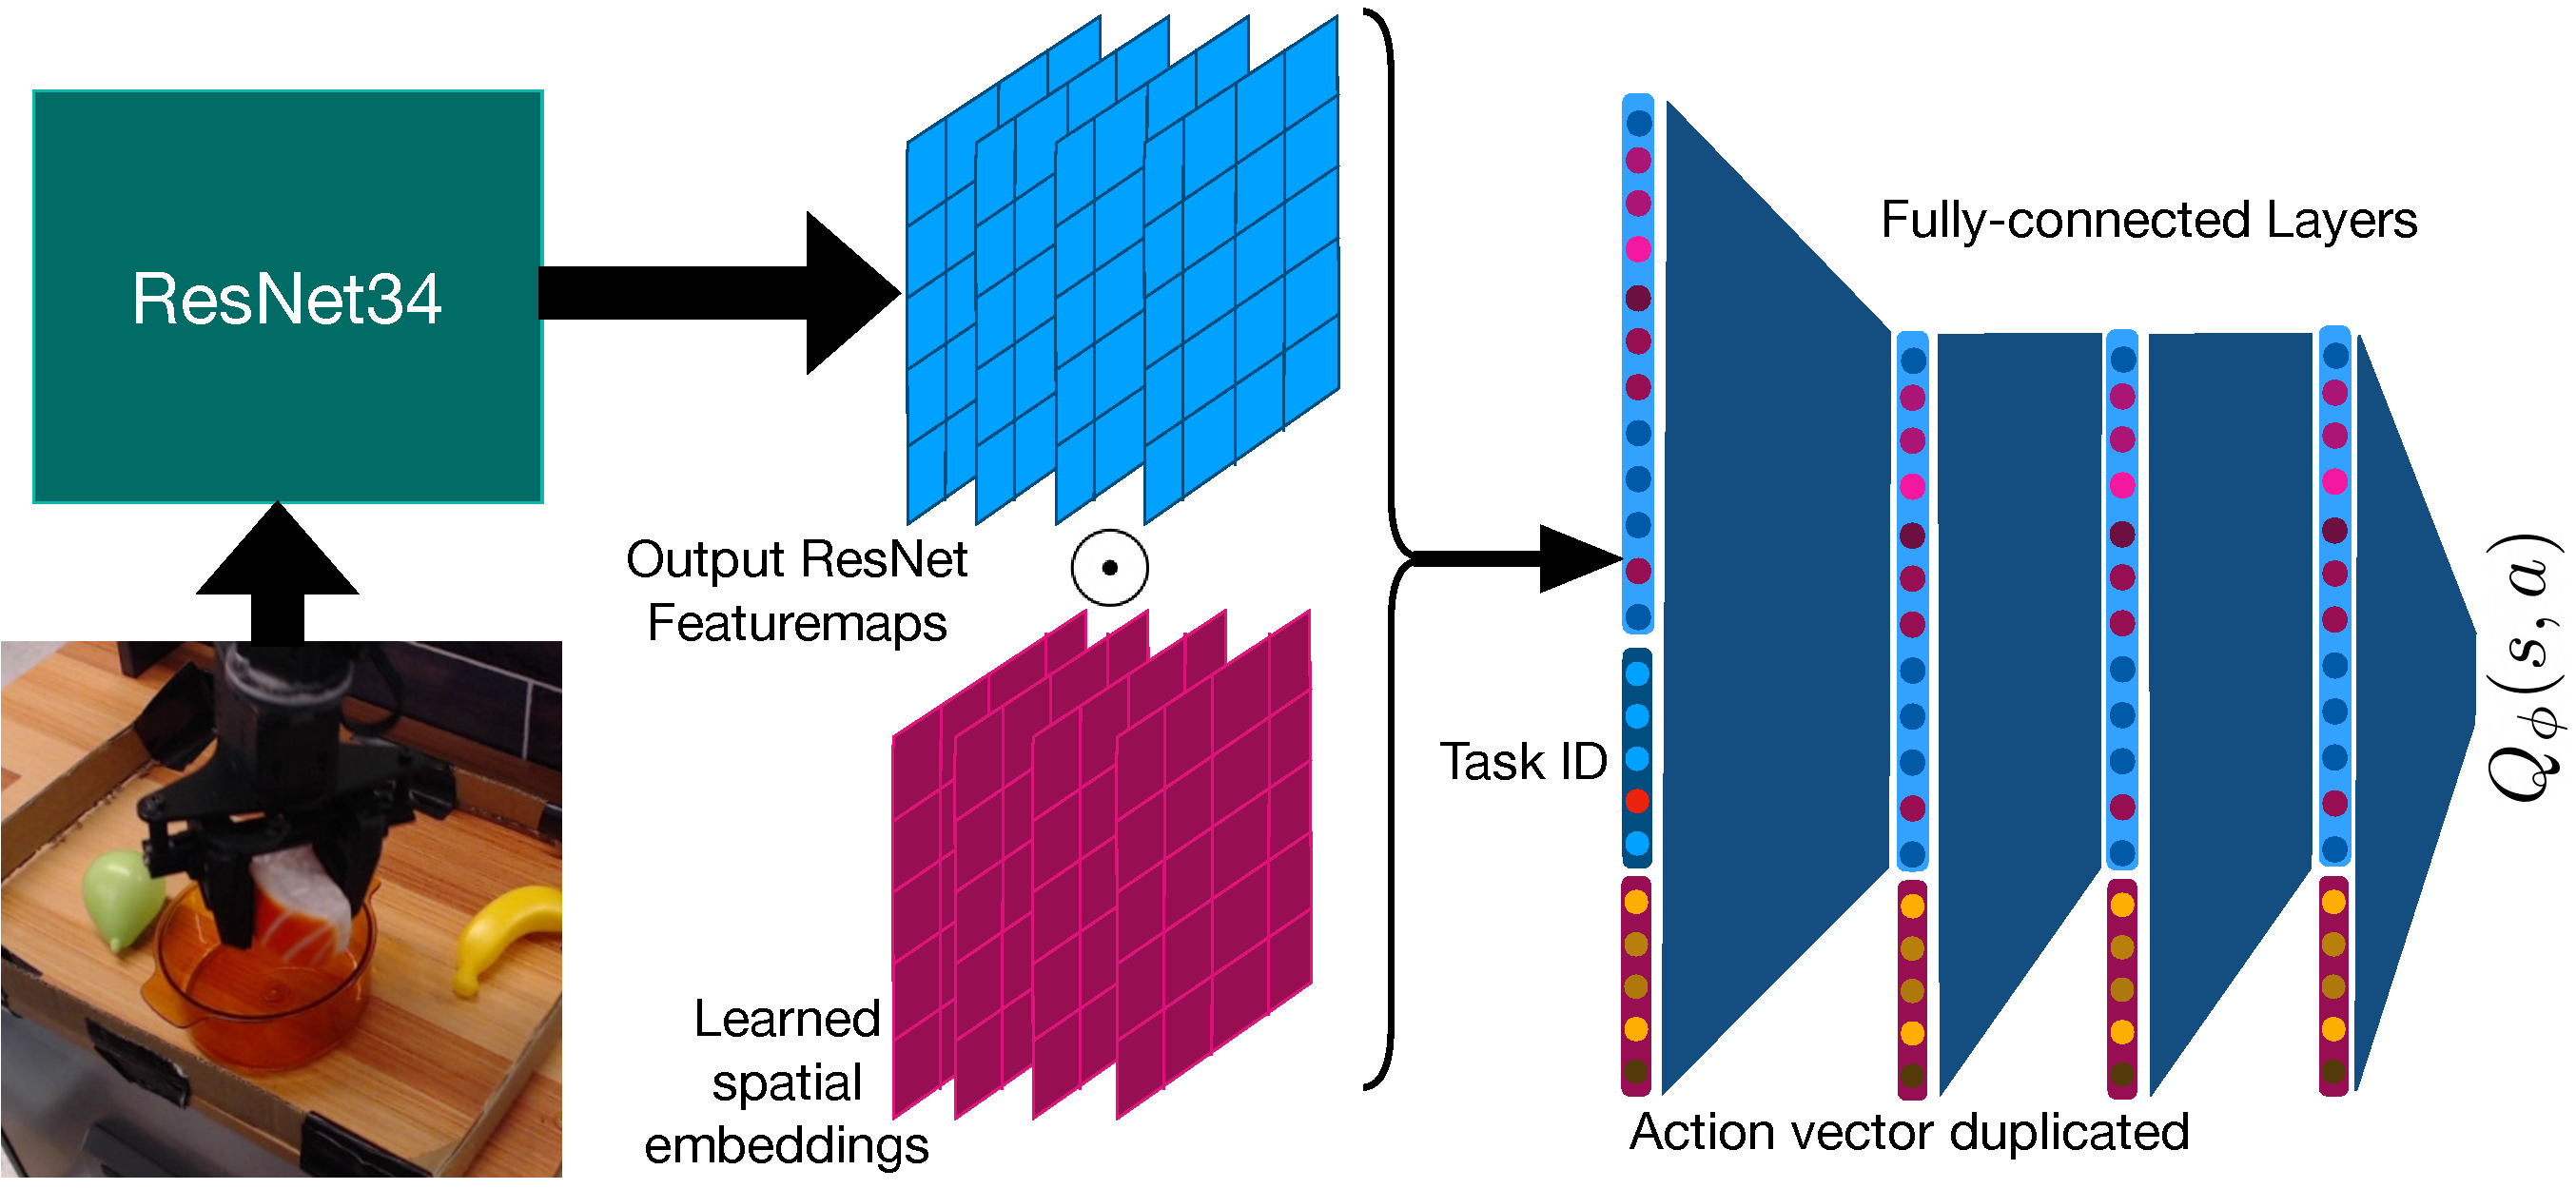
\includegraphics[width=0.75\linewidth]{chapters/ptr/architecture.pdf}
  \vspace{-0.2cm}
  \caption{\footnotesize{\textbf{Q-function architecture for \ptrmethodname.} The encoder is a ResNet34 with group normalization along with learned spatial embeddings (left). The decoder (right) is a MLP with the action vector duplicated and passed in at each layer. A one-hot task identifier is also passed into the input of the decoder.}}
  \vspace{-0.3cm}
  \label{fig:arch}
\end{figure}

\niparagraph{\large{\textbf{Policy and Q-function architectures}}}

Perhaps the most crucial design decision for our approach is the neural network architecture for representing $\pi^\text{off}$ and $Q^\text{off}$. Since we wish to fine-tune the policy for different tasks, we must use high-capacity neural network models for representing the policy and the Q-function. We experimented with a variety of standard (high-capacity) architectures for vision-based robotic RL. This includes standard convolutional architectures~\citep{singh2020cog} and IMPALA architectures~\citep{espeholt2018impala}. However, we observed in Figure~\ref{fig:scaling_ptr} that these {standard models were unable to effectively handle the diversity of the pre-training data} and performed poorly.
Then, we attempted to utilize standard ResNets~\citep{resnet} (ResNet-18, Resnet-34, and their adaptations to imitation problems from \citet{ebert2021bridge}) to represent $Q_\phi$, but faced divergence challenges similar to prior efforts that use batch normalization~\citep{bjorck2021towards,2019arXiv190205605B} in the Q-network. Batch normalization layers are known to be hard to train with TD-learning~\citep{2019arXiv190205605B} and, therefore, by replacing batch normalization layers with \textcolor{brown}{\textbf{group normalization}} layers~\citep{wu2018group}, we were able to address such divergence issues.
See Appendix~\ref{app:design} for quantitative studies comparing these choices. Unlike prior work~\citep{lee2022multi}, we observed that with group normalization, we attain favorable scaling properties of \ptrmethodname: the more the parameters, the better the performance as shown in Figure~\ref{fig:scaling_ptr}.
We also observed that choosing an appropriate method for converting the three-dimensional feature-map tensor produced by the ResNet into a one-dimensional embedding plays a crucial role for learning accurate Q-functions and obtaining functioning policies. Unlike standard ResNet architectures for supervised learning, simply utilizing global average pooling (as used in many classification architectures) performs poorly. Instead we point-wise multiply the learned feature-map with a 3-dimensional parameter tensor before computing sums over the spatial dimensions which allows the network to explicitly encode spatial information. {We refer to this technique as ``\textcolor{brown}{\textbf{learned spatial embeddings}}''}. An illustration of this architecture is provided in \autoref{fig:arch}. As detailed in Appendix~\ref{app:design}, Table~\ref{tab:spatial}, {we find that utilizing this technique leads to improved performance}.

Next, we found that a Q-function $Q_\phi(\bs, \mathbf{a})$ obtained by running na\"ive multi-task CQL on the demonstration data tends to not use the action input $\mathbf{a}$ effectively, due to strong correlations between $\bs$ and $\mathbf{a}$ in the data, which is almost always the case for narrow, human demonstrations. As a result, policy improvement against such a Q-function overfits to these correlations, producing poor policies. To resolve this issue, we modified the architecture of Q-network to \textcolor{brown}{\textbf{pass the action \textbf{\textit{$\mathbf{a}$}} as input to every fully-connected layer}} which, as shown in \autoref{fig:arch} and {Appendix~\ref{app:design}}, {Table~\ref{tab:action_sep}}), greatly alleviates the issue {and significantly improves over na\"ive CQL}. 


\niparagraph{\large{\textbf{Cross-validation during offline fine-tuning}}} 

As we wish to learn task-specific policies that do not overfit to small amounts of data, we must apply the right number of gradient steps during fine-tuning: too few gradient steps will produce policies that do not succeed at the target tasks, while too many gradient steps will give policies that have likely lose the generalization ability of the pre-trained policy. {To handle this trade-off, we adopt the following heuristic as a loose guideline:} we run fine-tuning for many iterations while also plotting the learned Q-values over a held-out dataset of trajectories from the target task as seen in Figure~\ref{fig:moreexreb}. Then for evaluation, we pick the checkpoints that presented a Q-function with the Q-values appearing closest to having a monotonically increasing trend in a trajectory. This is a \emph{relative} guideline and must be performed within the checkpoints observed within a run. The reason for this heuristic choice is that a valid Q-function must be a valid estimator for discounted return, and hence, it must increase over time-steps of a trajectory for a given task.  Of course, this heuristic does not hold for arbitrary sub-optimal offline data, but all of our data comes from human-collected demonstrations. In principle, this heuristic can be wrapped into a metric quantifying degree of monotonicity of the Q-value curve in Figure~\ref{fig:moreexreb}, but in our experiments, we felt this was not necessary: as we show below, we were able to narrow down the checkpoints to essentially one or at most, two checkpoints by just visual inspection. Of course, designing an accurate metric would be helpful for future work. We present two worked-out examples of our checkpoint selection strategy for two tasks from Scenario 1 and Scenario 3 in Figure~\ref{fig:moreexreb}. Observe that checkpoints early in training exhibit Q-values that fluctuate arbitrarily at the beginning of training, which is clearly non-monotonic. This is because of the lack of sufficient gradient steps for fine-tuning the target task. Once sufficient gradient steps are performed, the Q-values visibly improve on the monotonicity property. Training further leads to much flatter Q-values, that are visibly less monotonic. 


\begin{figure}[h]
\centering
  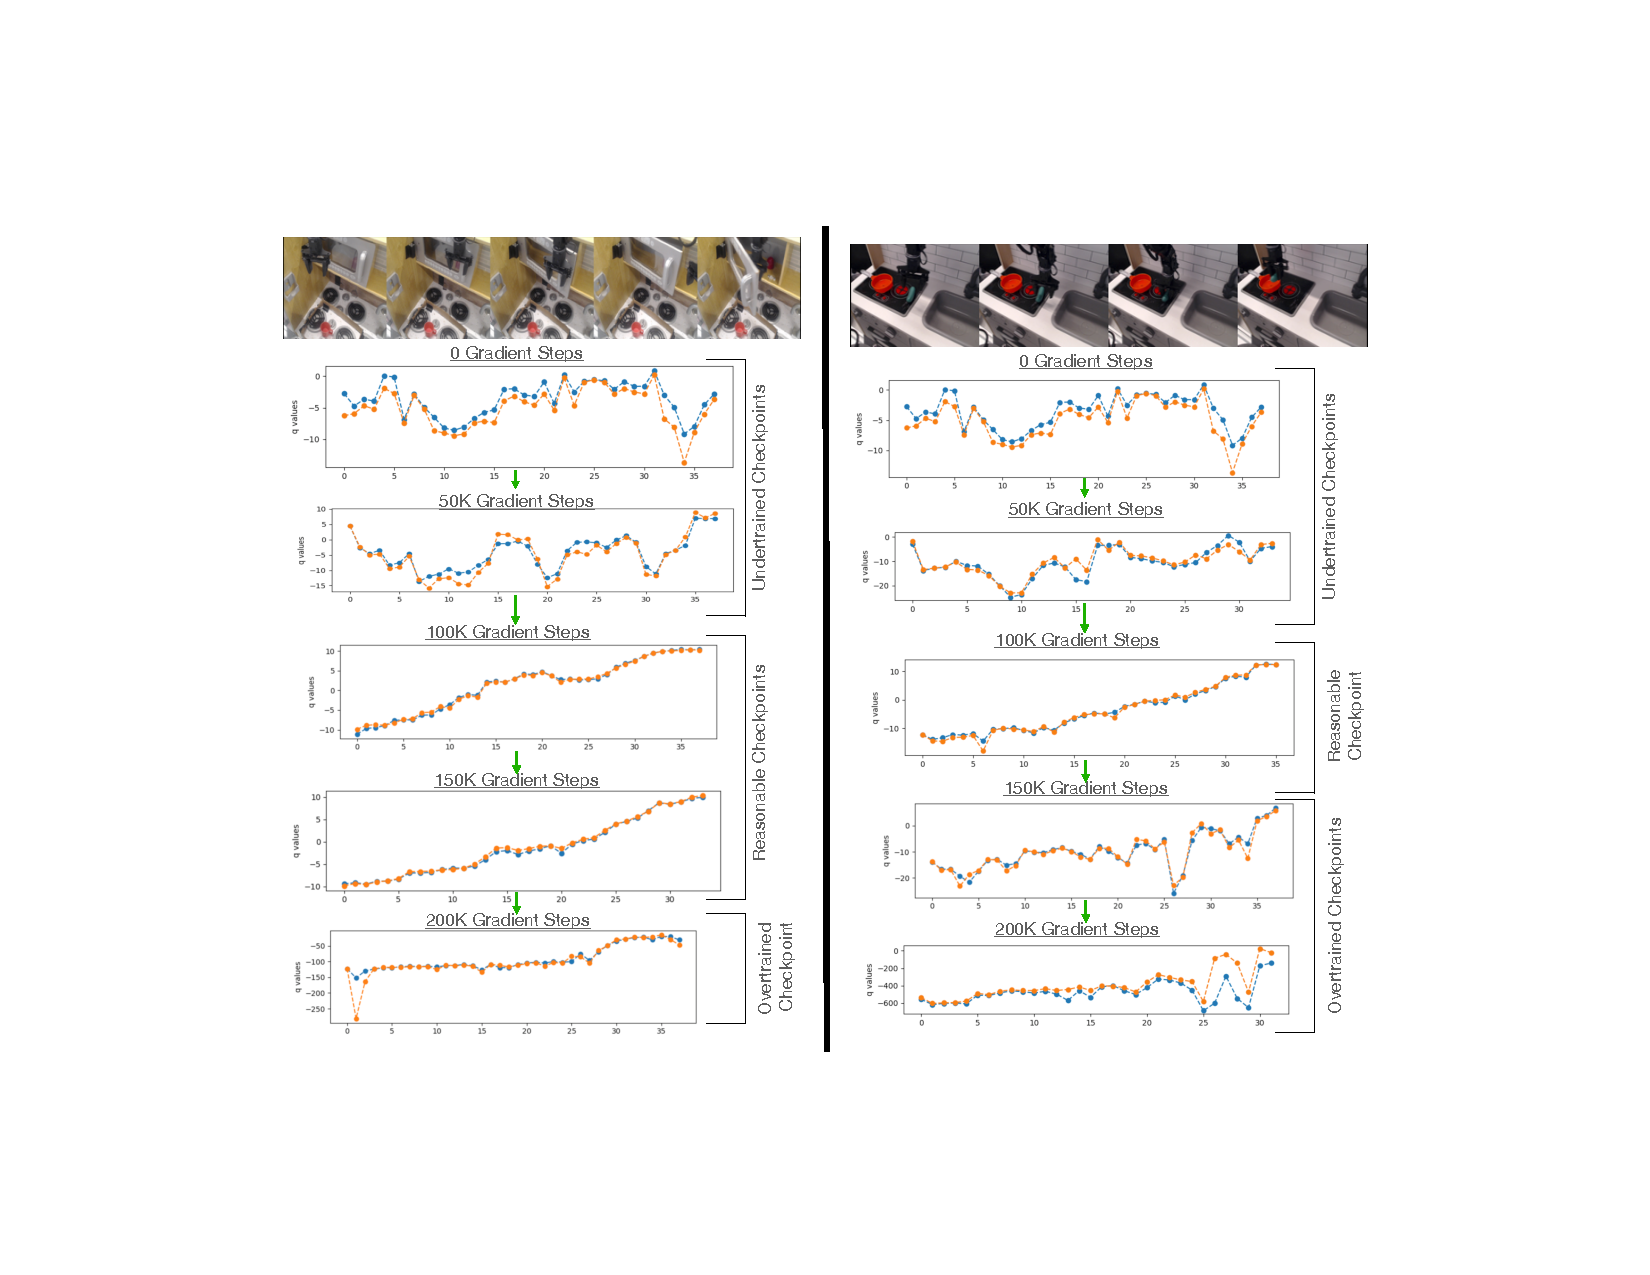
\includegraphics[width=0.6\linewidth]{chapters/ptr/Fig_rebuttal.pdf}
  \vspace{-0.1cm}
  \caption{\footnotesize \textbf{Evolution of Q-values on the target task over the process of fine-tuning with \ptrmethodname.} Observe that while the learned Q-values on \emph{held-out} trajectories from the dataset just at the beginning of Phase 2 (fine-tuning) do not exhibit a roughly increasing trend, we choose to evaluate those checkpoints of \ptrmethodname that exhibit a visible more increasing trend in the Q-values despite having access to only 10 demonstrations for these target tasks.}
  \label{fig:moreexreb}
  \vspace{-0.1cm}
\end{figure}

To validate this mechanism, in Figure~\ref{fig:validation_door} we present a film-strip of a sample evaluation of a good and a poor checkpoint as identified by the cross-validation strategy mentioned above. We observe that the checkpoint with more flat Q-values fails to solve the door opening task, whereas the one with a visibly increasing Q-value trend solves the task.

\begin{figure}[h]
\centering
\vspace{-0.2cm}
  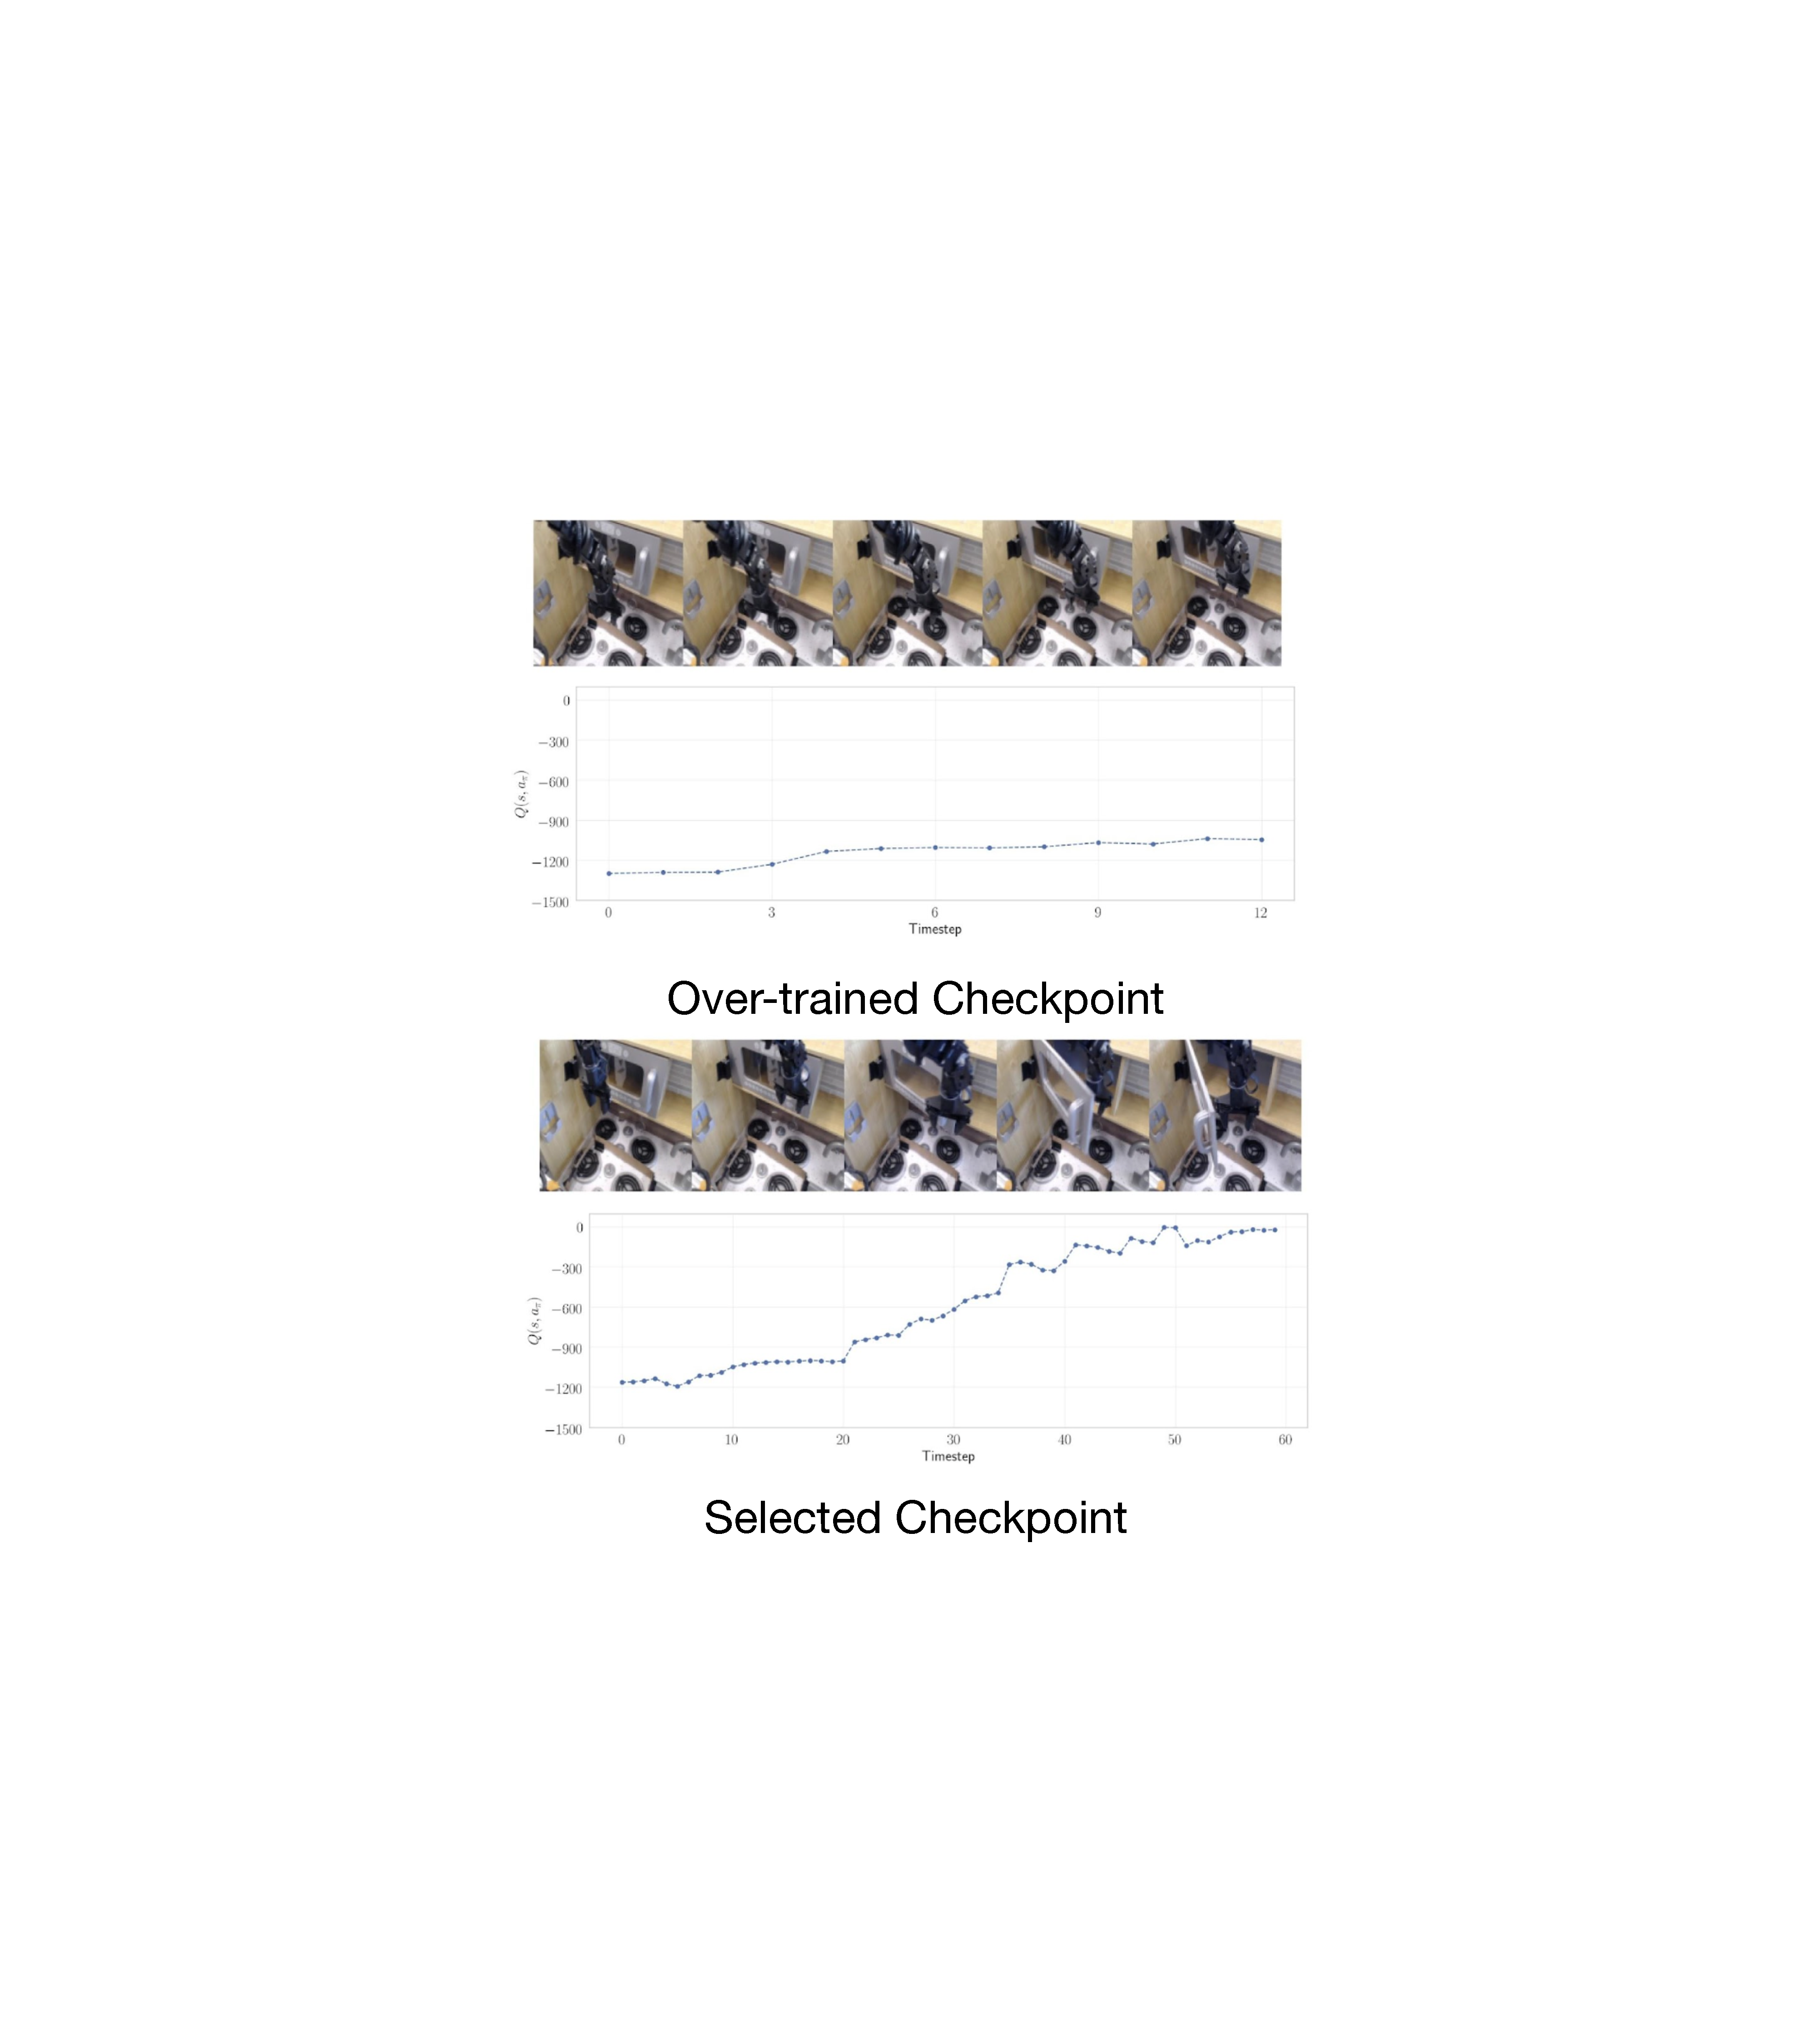
\includegraphics[width=0.6\linewidth]{chapters/ptr/fig_chkpt.pdf}
  \vspace{-0.1cm}
  \caption{\footnotesize \textbf{Performance evaluation of a selected and over-trained checkpoint of \ptrmethodname.} We validate our checkpoint selection mechanism on the door opening task. An over-trained checkpoint with nearly flat Q-values fails to solve the task, whereas a checkpoint with visibly increasing Q-values solves the task.}
  \label{fig:validation_door}
  \vspace{-0.2cm}
\end{figure}

\niparagraph{\large{\textbf{Reward specification}}} 

In this paper, we aim to pre-train on existing robotic datasets, such as the Bridge Dataset~\citep{ebert2021bridge}, which consists of human-teleoperated demonstration data. Although the demonstrations are all successful, they are not annotated with any reward function. Perhaps an obvious choice is to label the last transition of each trajectory as success, and give it a +1 binary reward. However, in several of the datasets we use, there can be a 0.5-1.0 second lag between task completion and when the episode is terminated by the data collection. To ensure that a successful transition is not incorrectly labeled as $0$, we utilized the practical heuristic of annotating the last $n=3$ transitions of every trajectory with a reward of $+1$ and and annotated other states with a $0$ reward. We show in Appendix~\ref{app:exp_results} that this provided the best results. 
In principle, more complicated methods of reward labeling~\citep{eysenbach2021replacing} could be used. However, we found the presented rule to be simple and yet effective to learn good policies.

